\documentclass[11pt,a4paper]{article}
\usepackage[margin=1in]{geometry}
\usepackage{graphicx}
\usepackage{subcaption}
\usepackage{booktabs}
\usepackage{fancyhdr}
\usepackage{enumitem}

\pagestyle{fancy}
\fancyhf{}
\lhead{Laboratory Report}
\rhead{AI5707: PRML -- Lab Assignment 8}
\cfoot{Page \thepage}
\renewcommand{\headrulewidth}{0.4pt}

\setlist[itemize]{itemsep=2pt,topsep=3pt}
\setlist[enumerate]{itemsep=2pt,topsep=3pt}

\begin{document}

\begin{center}
{\LARGE \textbf{Classification and Dimensionality Reduction using PCA}}\\[6pt]
{\large Lab Assignment 8 Report}\\[6pt]
Shrawanthi P. (Roll No: 26120098) \quad Shreepriyadarshini RM. (Roll No: 26120099)\\[4pt]
10th November 2026
\end{center}

\section{Objective}
In this lab, we test four classifiers using Python and NumPy:
\begin{itemize}
  \item Gaussian Mixture Model (GMM)
  \item Linear Discriminant Analysis (LDA)
  \item K-Nearest Neighbours (KNN)
  \item Support Vector Machine (SVM)
  \item Four Datasets:
  \begin{itemize}
    \item \textbf{Synthetic Data:} 20,000 points in 16 dimensions for 2 classes.
    \item \textbf{MNIST Digits:} Grayscale handwritten images ($28 \times 28 = 784$ pixels) of digits 1, 8, and 9.
    \item \textbf{Image Features:} 3,000 samples of 36 pre-computed features from 5 classes.
    \item \textbf{TIDIGITS Audio:} 1,350 speech recordings of spoken digits 3, 7, and 9, represented by 39-D MFCC feature frames.
  \end{itemize}
\end{itemize}

\section{Workflow}
\begin{enumerate}
  \item \textbf{Split Data:} Split each dataset into train, validation, and test sets.
  \item \textbf{Scale Features:} Normalised features with the mean and standard deviation of the training set: $z = (x - \mu)/\sigma$.
  \item \textbf{Speech Setup:} We used two types of audio representations: (a) average all frames into one 78-D vector (mean and std), and (b) use all 39-D frames directly with a GMM.
  \item \textbf{PCA Projection:} Obtain the top $K$ directions with the highest variance in the training data, and map all data to $K$ dimensions.
  \item \textbf{Train and Test:} Trained and tested all four models on the original features and PCA features. Evaluate the performance using accuracy and confusion matrices.
\end{enumerate}

\section{Outputs, Results, and Observations}

\subsection{Synthetic Dataset (16-Dim vs. PCA 8-Dim)}
Split into 12,000 train, 4,000 validation, 4,000 test points. The number of features that are reduced by PCA is 16. 8 dimensions were retained accounting for 72.7\% of the variance.

\begin{table}[htbp]
\centering
\begin{tabular}{@{}lccccc@{}}
\toprule
\textbf{Classifier} & \textbf{Orig. Val} & \textbf{Orig. Test} & \textbf{PCA Val} & \textbf{PCA Test} & \textbf{Change ($\Delta$)} \\
\midrule
GMM & 96.88\% & 96.43\% & 95.47\% & 95.25\% & -1.18\% \\
LDA & 92.63\% & 92.85\% & 88.15\% & 88.15\% & -4.70\% \\
KNN & 99.40\% & 99.35\% & 96.90\% & 96.77\% & -2.58\% \\
SVM & 99.02\% & 98.78\% & 96.67\% & 96.65\% & -2.13\% \\
\bottomrule
\end{tabular}
\caption{Synthetic Dataset's Accuracies (16-Dim vs. PCA 8-Dim).}
\label{tab:synthetic_acc}
\end{table}

\begin{table}[htbp]
\centering
\begin{tabular}{@{}lcccc@{}}
\toprule
& \multicolumn{2}{c}{\textbf{Original Features (16-D)}} & \multicolumn{2}{c}{\textbf{PCA Features (8-D)}} \\
\cmidrule(lr){2-3} \cmidrule(lr){4-5}
\textbf{True Class} & \textbf{Pred. Class 0} & \textbf{Pred. Class 1} & \textbf{Pred. Class 0} & \textbf{Pred. Class 1} \\
\midrule
Class 0 & 1961 & 15 & 1902 & 74 \\
Class 1 & 11 & 2013 & 55 & 1969 \\
\bottomrule
\end{tabular}
\caption{KNN confusion matrix result of 4,000 points of test.}
\label{tab:synthetic_cm}
\end{table}

\begin{figure}[htbp]
\centering
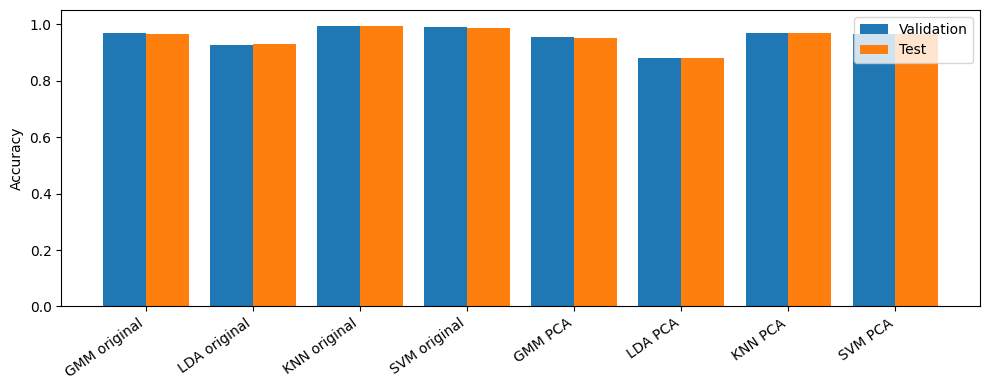
\includegraphics[width=0.88\textwidth]{synthetic_output.png}
\caption{Synthetic Dataset (16-D vs. PCA 8-D) --- Validation and Test Accuracies across Classifiers.}
\label{fig:synthetic_output}
\end{figure}

\noindent\textbf{Observations:}
\begin{itemize}
  \item If the classes have curved boundaries, then KNN (99.35\%) and SVM (98.78\%) are optimum. LDA is less accurate (92.85\%) due to its ability to only draw straight lines.
  \item All models performed with less accuracy when PCA was applied. The largest accuracy drop (-4.70\%) was shown by LDA because of the dropped dimensions useful informations were obtained to discriminate between the classes.
\end{itemize}

\subsection{MNIST Handwritten Digits (784-D vs. PCA 40-D)}
Digits 1, 8, and 9 have 21,660 in total, where the dataset was split into 14,833 train, 3,709 validation, and 3,118 test images. 784 pixels were reduced to 40 features by using PCA. The difference in fittings was 56.6\% of the variance that was retained from pixels.

\begin{table}[htbp]
\centering
\begin{tabular}{@{}lccccc@{}}
\toprule
\textbf{Classifier} & \textbf{Orig. Val} & \textbf{Orig. Test} & \textbf{PCA Val} & \textbf{PCA Test} & \textbf{Change ($\Delta$)} \\
\midrule
GMM & 94.10\% & 93.94\% & 91.20\% & 90.92\% & -3.02\% \\
LDA & 96.60\% & 96.54\% & 96.40\% & 96.34\% & -0.20\% \\
KNN & 98.40\% & 98.33\% & 98.30\% & 98.30\% & -0.03\% \\
SVM & 97.10\% & 96.99\% & 97.90\% & 97.82\% & +0.83\% \\
\bottomrule
\end{tabular}
\caption{Accuracies on MNIST digits 1, 8, and 9 (784-D vs. PCA 40-D).}
\label{tab:mnist_acc}
\end{table}

\begin{table}[htbp]
\centering
\begin{tabular}{@{}lcccc@{}}
\toprule
\textbf{True Digit} & \textbf{Pred. Digit 1} & \textbf{Pred. Digit 8} & \textbf{Pred. Digit 9} & \textbf{Recall} \\
\midrule
Digit 1 & 1129 & 5 & 1 & 99.47\% \\
Digit 8 & 2 & 958 & 14 & 98.36\% \\
Digit 9 & 8 & 23 & 978 & 96.93\% \\
\bottomrule
\end{tabular}
\caption{KNN confusion matrix for 3118 test images with 40 PCA features.}
\label{tab:mnist_cm}
\end{table}

\begin{figure}[htbp]
\centering
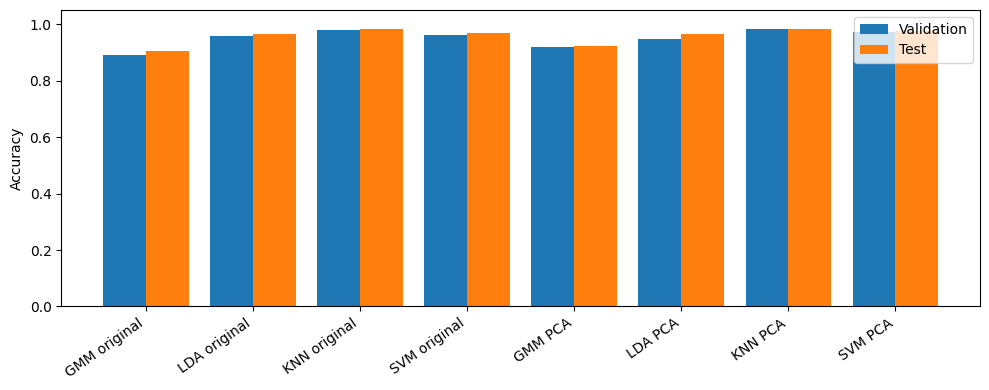
\includegraphics[width=0.88\textwidth]{MNIST_output.png}
\caption{MNIST Handwritten Digits (784-D vs. PCA 40-D) --- Accuracy and Latency Comparison.}
\label{fig:mnist_output}
\end{figure}

\noindent\textbf{Observations:}
\begin{itemize}
  \item The result of KNN is very precise on raw pixels (98.33\%). The data was reduced by 95\% using PCA, but KNN still achieves an accuracy of 98.30\% and runs much faster.
  \item By removing noisy background pixels, PCA is able to help SVM slightly (from 96.99\% to 97.82\%).
  \item The major errors occur between digits 8 and 9, where both have loops so the model got confused. Digit 1 has almost no mistakes.
\end{itemize}

\subsection{Image Features Dataset (36-Dim vs. PCA 12-Dim)}
This dataset has 3,000 samples with 5 classes (2,000 train, 500 val, 500 test). The features reduced from 36 to 12 using PCA (69.4\% variance kept).

\begin{table}[htbp]
\centering
\begin{tabular}{@{}lccccc@{}}
\toprule
\textbf{Classifier} & \textbf{Orig. Val} & \textbf{Orig. Test} & \textbf{PCA Val} & \textbf{PCA Test} & \textbf{Change ($\Delta$)} \\
\midrule
GMM & 43.40\% & 44.20\% & 43.20\% & 47.80\% & +3.60\% \\
LDA & 43.80\% & 43.20\% & 44.00\% & 44.20\% & +1.00\% \\
KNN & 43.40\% & 41.60\% & 40.60\% & 41.80\% & +0.20\% \\
SVM & 50.40\% & 51.60\% & 50.40\% & 49.60\% & -2.00\% \\
\bottomrule
\end{tabular}
\caption{Accuracies on Image Features (36-D vs. PCA 12-D).}
\label{tab:img_acc}
\end{table}

\begin{table}[htbp]
\centering
\begin{tabular}{@{}lcccccc@{}}
\toprule
\textbf{True Class} & \textbf{Pred. 0} & \textbf{Pred. 1} & \textbf{Pred. 2} & \textbf{Pred. 3} & \textbf{Pred. 4} & \textbf{Recall} \\
\midrule
Class 0 & 21 & 22 & 19 & 18 & 20 & 21.0\% \\
Class 1 & 0 & 82 & 4 & 10 & 4 & 82.0\% \\
Class 2 & 5 & 17 & 44 & 19 & 15 & 44.0\% \\
Class 3 & 10 & 6 & 12 & 59 & 13 & 59.0\% \\
Class 4 & 12 & 20 & 6 & 10 & 52 & 52.0\% \\
\bottomrule
\end{tabular}
\caption{SVM confusion matrix on 500 test samples on original features.}
\label{tab:img_cm}
\end{table}

\begin{figure}[htbp]
\centering
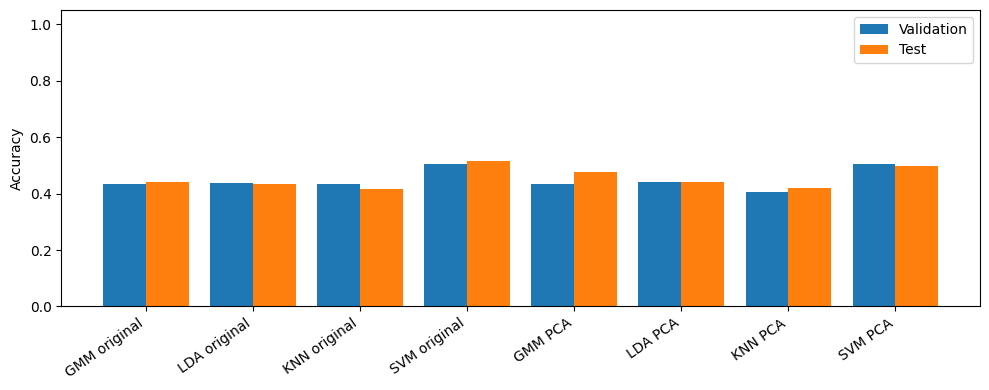
\includegraphics[width=0.88\textwidth]{image_feature_output.png}
\caption{Image Features Dataset (36-D vs. PCA 12-D) --- Classifier Accuracies (Val vs. Test).}
\label{fig:image_feature_output}
\end{figure}

\noindent\textbf{Observations:}
\begin{itemize}
  \item The 5 classes are highly overlapping, and the accuracies of all models are low (41\%--51\%). There was very little recall in Class 0 (21\%).
  \item The correlation between features were removed by using PCA in order to improve accuracy of GMM, this helps to stabilize the training of GMM (from 44.20\% to 47.80\%).
\end{itemize}

\subsection{TIDIGITS Spoken Digits (Digits 3, 7, 9)}
1,350 recordings (810 train, 270 val, 270 test). There were differences in comparison of 78-D summary vectors to the sequential 39-D frame GMM.

\begin{table}[htbp]
\centering
\begin{tabular}{@{}llccccc@{}}
\toprule
\textbf{Representation} & \textbf{Classifier} & \textbf{Orig. Val} & \textbf{Orig. Test} & \textbf{PCA Val} & \textbf{PCA Test} & \textbf{Change ($\Delta$)} \\
\midrule
78-D Summary & LDA & 37.41\% & 37.78\% & 31.48\% & 31.11\% & -6.67\% \\
78-D Summary & KNN & 29.26\% & 28.89\% & 32.96\% & 32.96\% & +4.07\% \\
78-D Summary & SVM & 38.89\% & 39.26\% & 32.96\% & 32.59\% & -6.67\% \\
Sequential Frames & Frame GMM & 99.26\% & 98.89\% & 99.26\% & 98.89\% & 0.00\% \\
\bottomrule
\end{tabular}
\caption{Analysis of TIDIGITS (78-D summary vectors vs. Frame GMM).}
\label{tab:tidigits_acc}
\end{table}

\begin{table}[htbp]
\centering
\begin{tabular}{@{}lcccccc@{}}
\toprule
& \multicolumn{3}{c}{\textbf{78-D Summary (SVM)}} & \multicolumn{3}{c}{\textbf{Sequential Frames (Frame GMM)}} \\
\cmidrule(lr){2-4} \cmidrule(lr){5-7}
\textbf{True Digit} & \textbf{Pred. 3} & \textbf{Pred. 7} & \textbf{Pred. 9} & \textbf{Pred. 3} & \textbf{Pred. 7} & \textbf{Pred. 9} \\
\midrule
Digit 3 & 30 & 26 & 34 & 89 & 1 & 0 \\
Digit 7 & 27 & 36 & 27 & 0 & 90 & 0 \\
Digit 9 & 25 & 25 & 40 & 2 & 0 & 88 \\
\bottomrule
\end{tabular}
\caption{Confusion matrices of 270 test audio files (90 for each digit).}
\label{tab:tidigits_cm}
\end{table}

\begin{figure}[htbp]
\centering
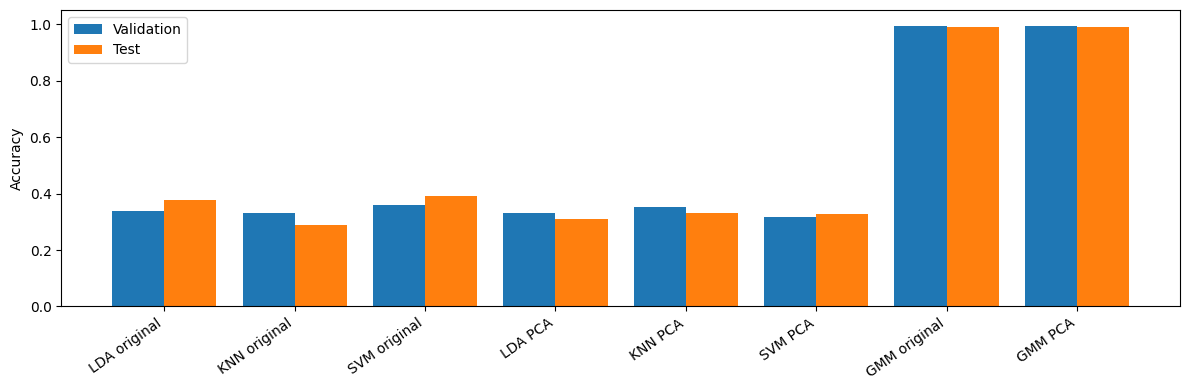
\includegraphics[width=0.92\textwidth]{tidigits_output.png}
\caption{TIDIGITS Spoken Digits (Digits 3, 7, 9) --- Summary Vectors vs. Sequential Frame GMM Accuracies.}
\label{fig:tidigits_output}
\end{figure}

\noindent\textbf{Observations:}
\begin{itemize}
  \item Taking an average over time was not very successful for LDA, KNN, and SVM ($\approx$29\%--39\%), which is almost equal to random guessing (33.3\%) since the sound order is lost.
  \item The highest result among all test methods is the accuracy of the frame-level GMM, which is 98.89\% for both original frames and 15-D PCA frames. The number of test files was 270, with only 3 misclassifications. It is essential to maintain individual sound frames for speech.
\end{itemize}

\section{Summary}
\begin{itemize}
  \item \textbf{Speech Needs Frames:} Even though speech features was classified correctly over short intervals, averaging those features reduced classification accuracy to approximately 35\%. However, evaluating individual frames with GMM gave an accuracy nearly 99\% accuracy.
  \item \textbf{Effects of PCA:} PCA works well when it removes noise (SVM on MNIST, GMM on image features). However, accuracy can be decreased when the dropped features contain meaningful information (Synthetic data).
  \item \textbf{Speed Gain:} On MNIST, PCA reduced the number of features from 784 to 40, significantly reducing the computation time for KNN with almost no change in accuracy (98.33\% to 98.30\%).
  \item \textbf{Linear vs. Non-linear:} KNN and SVM perform better than LDA when class boundaries are non-linear or curved.
\end{itemize}

\end{document}
